
\section{Основные элементы теплогидравлического кода}
\label{sec:section1}
Теплогидравлический код предназначен для расчёта динамики поведения основных параметров сжимаемого и несжимаемого теплоносителя в теплогидравлических контурах с произвольной топологией. В нём решаются уравнения сохранения массы, импульса и энергии для жидкости (в односкоростном приближении), а также нестационарные уравнения теплопроводности для тепловых структур (стенок каналов), в том числе с учётом теплового излучения между цилиндрическими стенками. Основой является одномерная нестационарная гомогенная модель течения сжимаемой жидкости. 

Код является внешней подключаемой в виде DLL-библиотек программой для Sim\-In\-Tech и работает совместно с ним, хотя принципиально может быть запущен отдельно. В графической подсистеме SimInTech пользователь из блоков набирает теплогидравлическую расчётную схему. Далее при инициализации задачи автоматически выполняется анализ набранной схемы и готовится файл расчётного задания для теплогидравлического кода. В коде осуществляется расчёт основных параметров (расходов, температур, давлений и т. д.) в элементах схемы, а отображение текущих значений и построение графиков осуществляется в графической оболочке SimInTech. 

В нодализационной схеме циркуляционный контур разбивается на расчётные ячейки. Расчётной ячейкой (контрольным объёмом) называется фиксированный в пространстве фрагмент потока теплоносителя, ограниченный поверхностями конструкций, формирующих поток. Граница между смежными (соседними) расчётными ячейками называется гидравлической связью. В каждой расчётной ячейке описывается теплогидравлика однофазного или двухфазного теплоносителя в сосредоточенных параметрах с использованием гомогенной модели. Скалярные характеристики потока (давление, энтальпия) определяются относительно центров ячеек из уравнений сохранения массы и энергии, а векторные (скорости) рассчитываются в гидравлических связях ячеек из уравнений сохранения импульса. Расчётные ячейки обмениваются массой и энергией с соседними ячейками посредством конвекции через гидравлические связи, а также обмениваются тепловой энергией со стенками каналов. Схема разбиения канала на контрольные объёмы показана на рисунке~\ref{fig11}.

\begin{figure}[ht]
\abovecaptionskip=2pt
\centering{
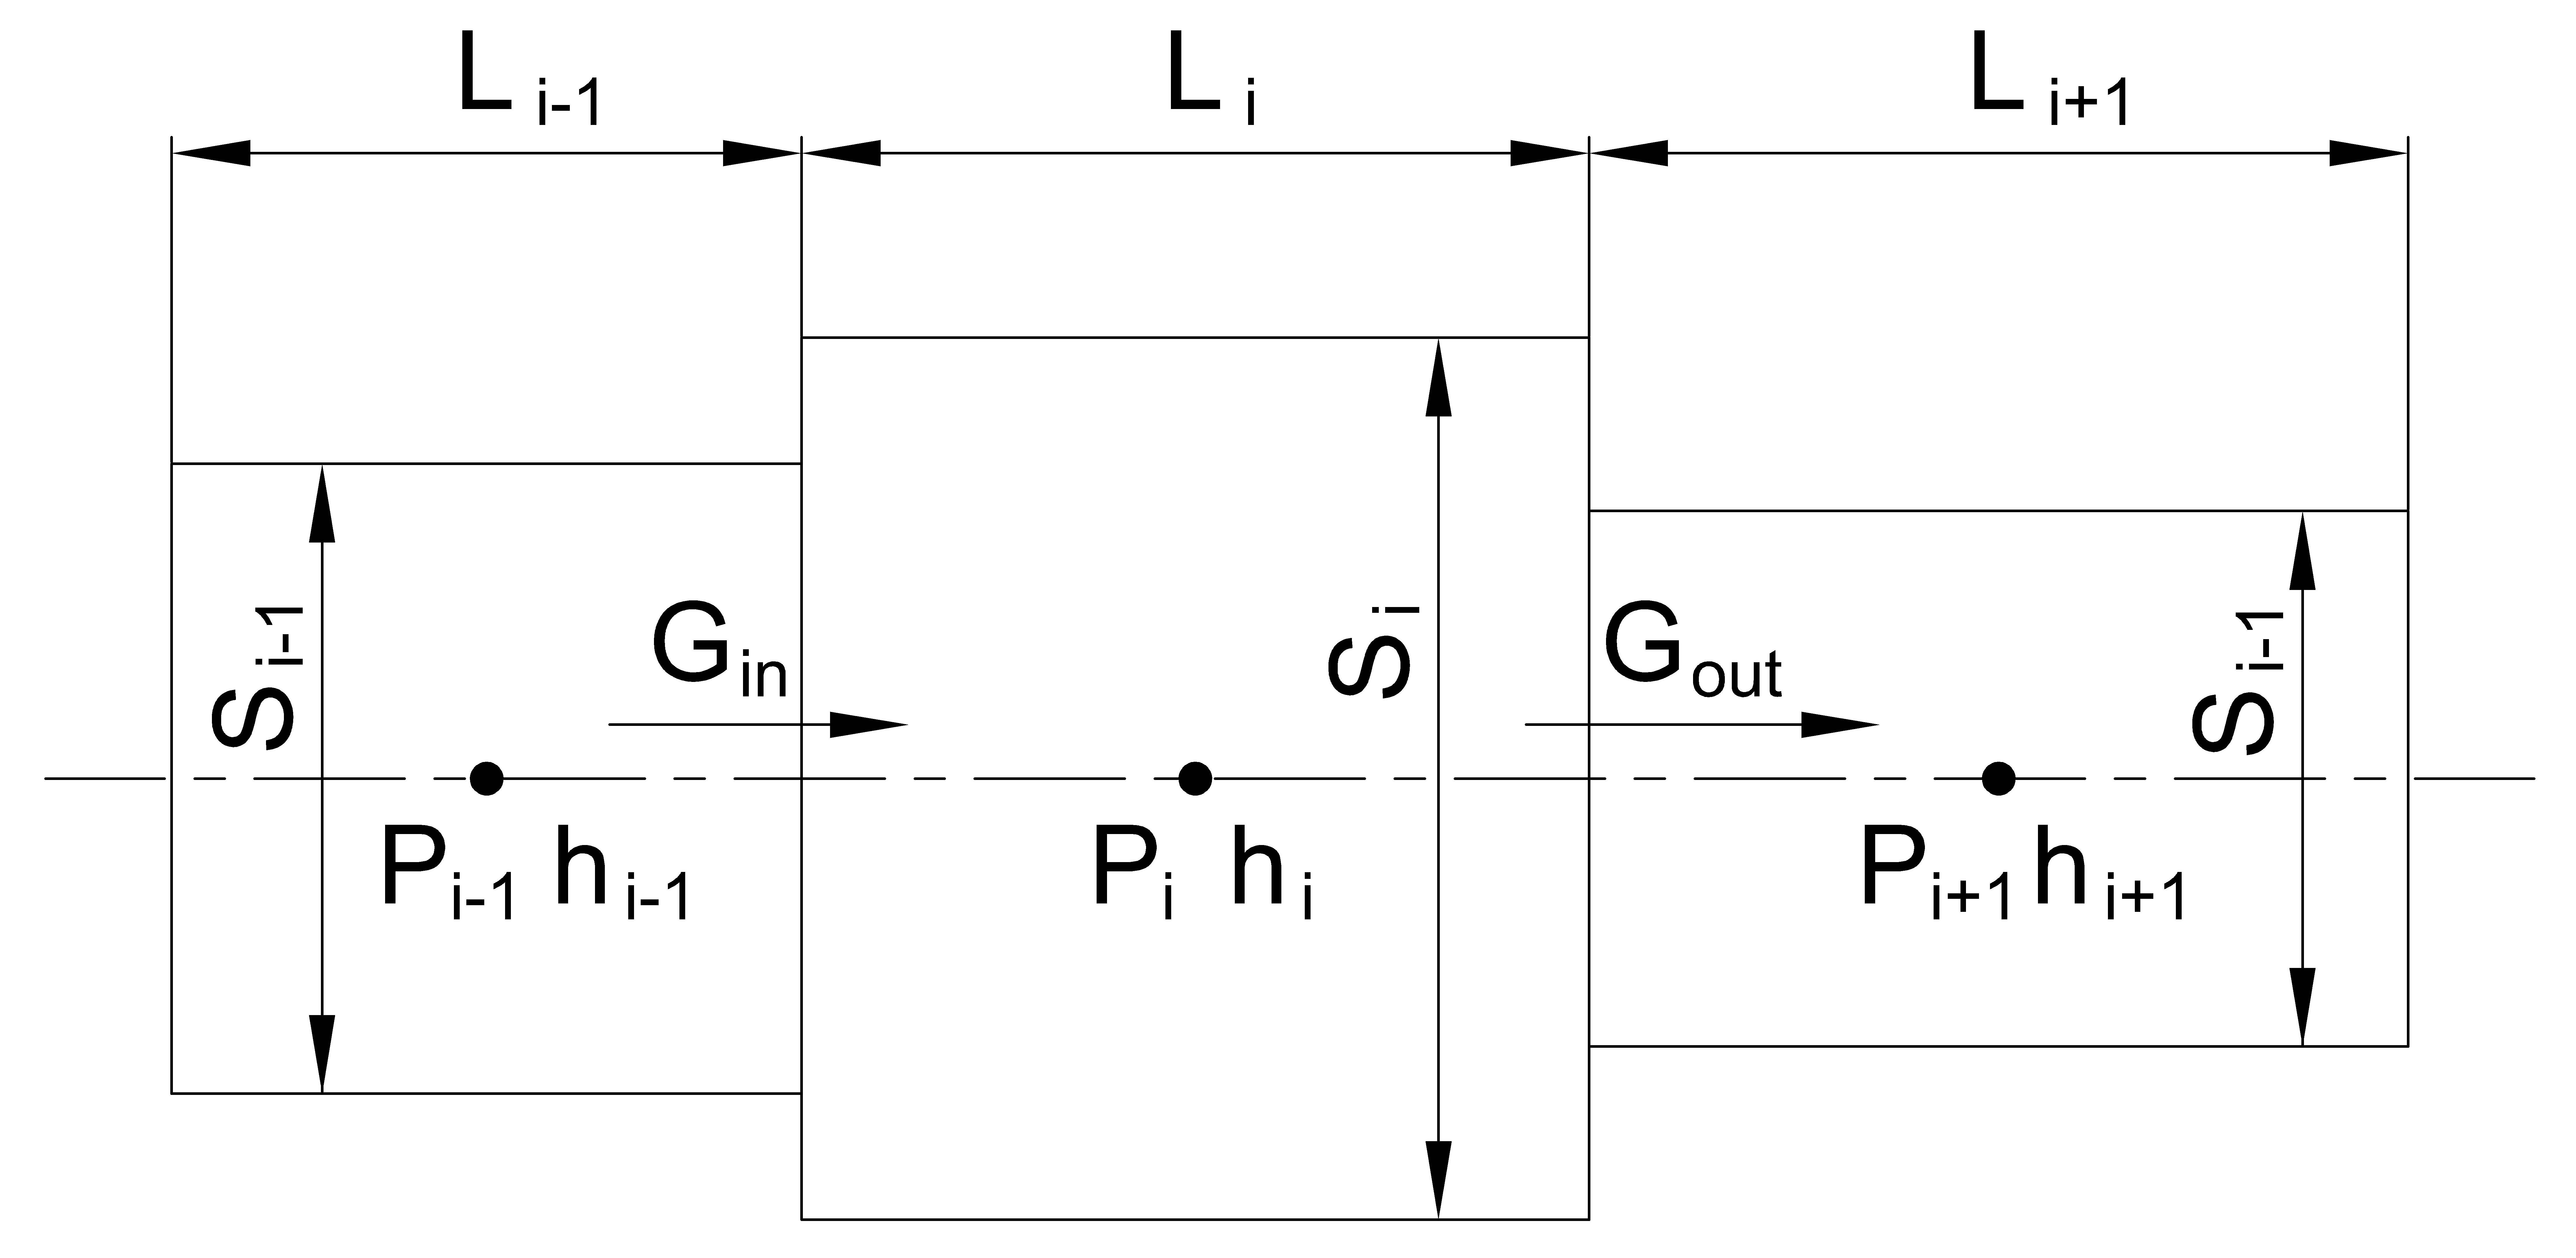
\includegraphics[width=1.0\linewidth]{KO_channel_differ.jpg} 
\caption{\textsc{Схема разбиения канала на контрольные объёмы}}\label{fig11}
}
\end{figure}

Граничная ячейка (граничный узел) отличается от обычной расчётной ячейки тем, что скалярные величины в ней известны (могут либо задаваться пользователем как функции времени, либо рассчитываться в специализированных модулях или в смежных задачах при помощи описываемого теплогидравлического модуля) и требуется рассчитывать только векторные величины в гидравлических связях.

Цепочка последовательно соединённых расчётных ячеек называется каналом. В каналах задается положительное направление движения теплоносителя, которое определяет положительное направление движения в гидравлических связях расчётных ячеек, составляющих канал. Если вычисленная скорость имеет противоположное направление, она будет иметь отрицательное значение. 
Соединение каналов возможно посредством другого элемента нодализационной схемы --- внутреннего узла, который представляет собой расчётную ячейку, которая может содержать два и более соединений. Множество расчётных ячеек, находящихся между двумя узлами, называется ребром. 

Кроме граничной ячейки воздействие различных внешних по отношению к рассматриваемому циркуляционному контуру систем можно отразить через элемент нодализационной схемы --- подпитку. Источник (сток) массы задаёт расходы и энтальпии, поступающие в любую расчётную ячейку из внешних по отношению к контуру систем или уходящие из расчётной ячейки ячейки во внешнюю систему. Подпитка предназначена для моделирования незамкнутых контуров с заданным расходом теплоносителя.
\newpage











